\chapter{Linear Regression}


\section{Representation}

\begin{equation}
y=f(x)=\vec{w}^T\vec{x}+b \quad , \vec{x} \in \mathbb{R}^D, y \in \mathbb{R}
\end{equation}

If we extend $\vec{x}^T=(1,x_1,x_2,\cdots,x_D),\vec{w}^T=(b,w_1,w_2,\cdots,w_D)$, then
\begin{equation}
y=f(x)=\vec{w}^T\vec{x}
\end{equation}


\begin{figure}[hbtp]
\centering
    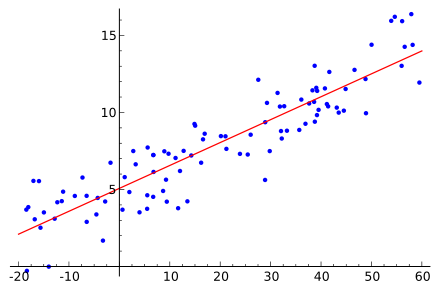
\includegraphics[scale=.50]{Linear-regression.png}
\caption{Example of simple linear regression, \\ which has one independent variable, from Wikipedia}
\label{fig:Linear-regression} 
\end{figure}


\section{Evaluation}

\begin{eqnarray}
R_{emp}(f) &=& \frac{1}{2N}\sum\limits_{i=1}^N \left(y-f(\vec{x})\right)^2=\frac{1}{2N}\sum\limits_{i=1}^N \left(y-\vec{w}^T\vec{x}\right)^2 \\
J(\vec{w}) &\triangleq& R_{emp}(f)
\end{eqnarray}

Prerequisite: define error term $\epsilon_i \triangleq y_i-\vec{w}^T\vec{x}_i$, $\epsilon_i$ are IID (independently and identically distributed) according to a Gaussian distribution. 


\section{Optimization}


\subsection{Normal Equation}
When dataset is small, use Normal Equation to compute \vec{w} directly.

\begin{equation}
y=f(x)=\vec{w}^T\vec{x} \vec{w}=(X^TX)^{-1}X^T\vec{y}
\end{equation}
where
\begin{eqnarray*}
X &=& \left[\vec{x}_1^T,\vec{x}_2^T,\cdots,\vec{x}_N^T\right]^T \\
\vec{y} &=& (y_1,y_2,\cdots,y_N)^T
\end{eqnarray*}


\begin{proof}
We now state without proof some facts of matrix derivatives (we won’t need all of these at this section).
\begin{eqnarray}
trA &\triangleq& \sum\limits_{i=1}^n A_{ii} \nonumber \\
\frac{\partial}{\partial A}AB &=& B^T \\
\frac{\partial}{\partial A^T}f(A) &=& \left[\frac{\partial}{\partial A}f(A)\right]^T \label{eqn:matrix-1} \\
\frac{\partial}{\partial A}ABA^TC &=& CAB+C^TAB^T \label{eqn:matrix-2} \\
\frac{\partial}{\partial A}|A| &=& |A|(A^{-1})^T
\end{eqnarray}

\begin{eqnarray*}
J(\vec{w}) &=& \frac{1}{2N}(X\vec{w}-\vec{y})^T(X\vec{w}-\vec{y}) \\
\frac{\partial J}{\vec{w}} &=& \frac{1}{2N} \frac{\partial}{\vec{w}} (\vec{w}^TX^TX\vec{w}-\vec{w}^TX^T\vec{y}-\vec{y}^TX\vec{w}+\vec{y}^T\vec{y}) \\
                           &=& \frac{1}{2N} \frac{\partial}{\vec{w}} (\vec{w}^TX^TX\vec{w}-\vec{w}^TX^T\vec{y}-\vec{y}^TX\vec{w}) \\
						   &=& \frac{1}{2N} \frac{\partial}{\vec{w}} tr(\vec{w}^TX^TX\vec{w}-\vec{w}^TX^T\vec{y}-\vec{y}^TX\vec{w}) \\
						   &=& \frac{1}{2N} \frac{\partial}{\vec{w}} (tr\vec{w}^TX^TX\vec{w}-2tr\vec{y}^TX\vec{w})
\end{eqnarray*}

Combining Equations \eqref{eqn:matrix-1} and \eqref{eqn:matrix-2}, we find that 
\begin{equation*}
\frac{\partial}{\partial A^T}ABA^TC = B^TA^TC^T+BA^TC
\end{equation*}

Let $A^T=\vec{w}, B=B^T=X^TX$, and $C=I$, Hence,
\begin{eqnarray*}
\frac{\partial J}{\vec{w}} &=& \frac{1}{2N} (X^TX\vec{w}+X^TX\vec{w} -2X^T\vec{y}) \\
						   &=& \frac{1}{2N} (X^TX\vec{w} - X^T\vec{y}) \\
\frac{\partial J}{\vec{w}} &=& 0 \Rightarrow X^TX\vec{w} - X^T\vec{y} =0 \\
X^TX\vec{w} &=& X^T\vec{y} \\
\vec{w} &=& (X^TX)^{-1}X^T\vec{y}
\end{eqnarray*}
\end{proof}


\subsection{SGD}
When dataset is large, use stochastic gradient descent(SGD).

\begin{eqnarray}
\dfrac{\partial}{\partial \vec{w}}J(\vec{w}) &=& \left[y_i - f(\vec{x}_i) \right]\vec{x}_i \\
\vec{w} &=& \vec{w} - \alpha\dfrac{\partial}{\partial \vec{w}}f(\vec{w}) \nonumber \\
        &=& \vec{w} - \alpha\left[y_i - f(\vec{x}_i) \right]\vec{x}_i
\end{eqnarray}
